%==============================================================================%
\chapter{Applications and Visualisations} \label{chapter:application}
%==============================================================================%
This chapter serves as a gallery of possible applications that can arise from the data generated from the Smart Street Sensor project.  As was  seen in Chapter \ref{chapter:literature}, availability of granular, longitudinal data on the movement and distribution of people at such spatial extent has numerous uses in various fields of study. This chapter first starts by looking at the use of the data in understanding the broad footfall landscape of the United Kingdom (UK), deriving sample insights on how retail footfall in the UK has been performing for the past couple of years. The sample analysis was done on various levels, from the national level to individual locations.

%------------------------------------------------------------------------------%
\section{Footfall Landscape of United Kingdom}
%------------------------------------------------------------------------------%
Figure \ref{figure:applications:footfall:index} shows the weekly footfall index of the UK from 2017 to 2018. In addition to showing larger trends, this index also shows sudden short term changes such as during the storm in February 2018. Figure \ref{figure:applications:cities:change} shows the spatial distribution of footfall change in the UK between these two years across cities, showing the growth and decline of retail in the cities of West Bromwich and Ipswich. These changes could be further looked at in temporal detail as shown in Figure \ref{figure:applications:cities:month}. The difference in even smaller intra-day patterns which show the nature of the economies of cities can also be inferred by their data profiles as shown in Figure \ref{figure:applications:cities:profiles}.

Figure  shows the weekly footfall index of UK through 2017 to 2018 which in addition to showing larger trends also shows sudden short term changes such as week during the storm in Feb 2018. Figure  shows the spatial distribution of the footfall change in UK between these two years across cities showing the growth and decline of retail in the cities of West Bromwich and Ipswich. These changes could be further looked at in detail temporally as shown in figure even smaller intra day patterns showing the nature of the economies of cities can also be inferred by their data profiles as shown in figure .

\begin{figure*}
  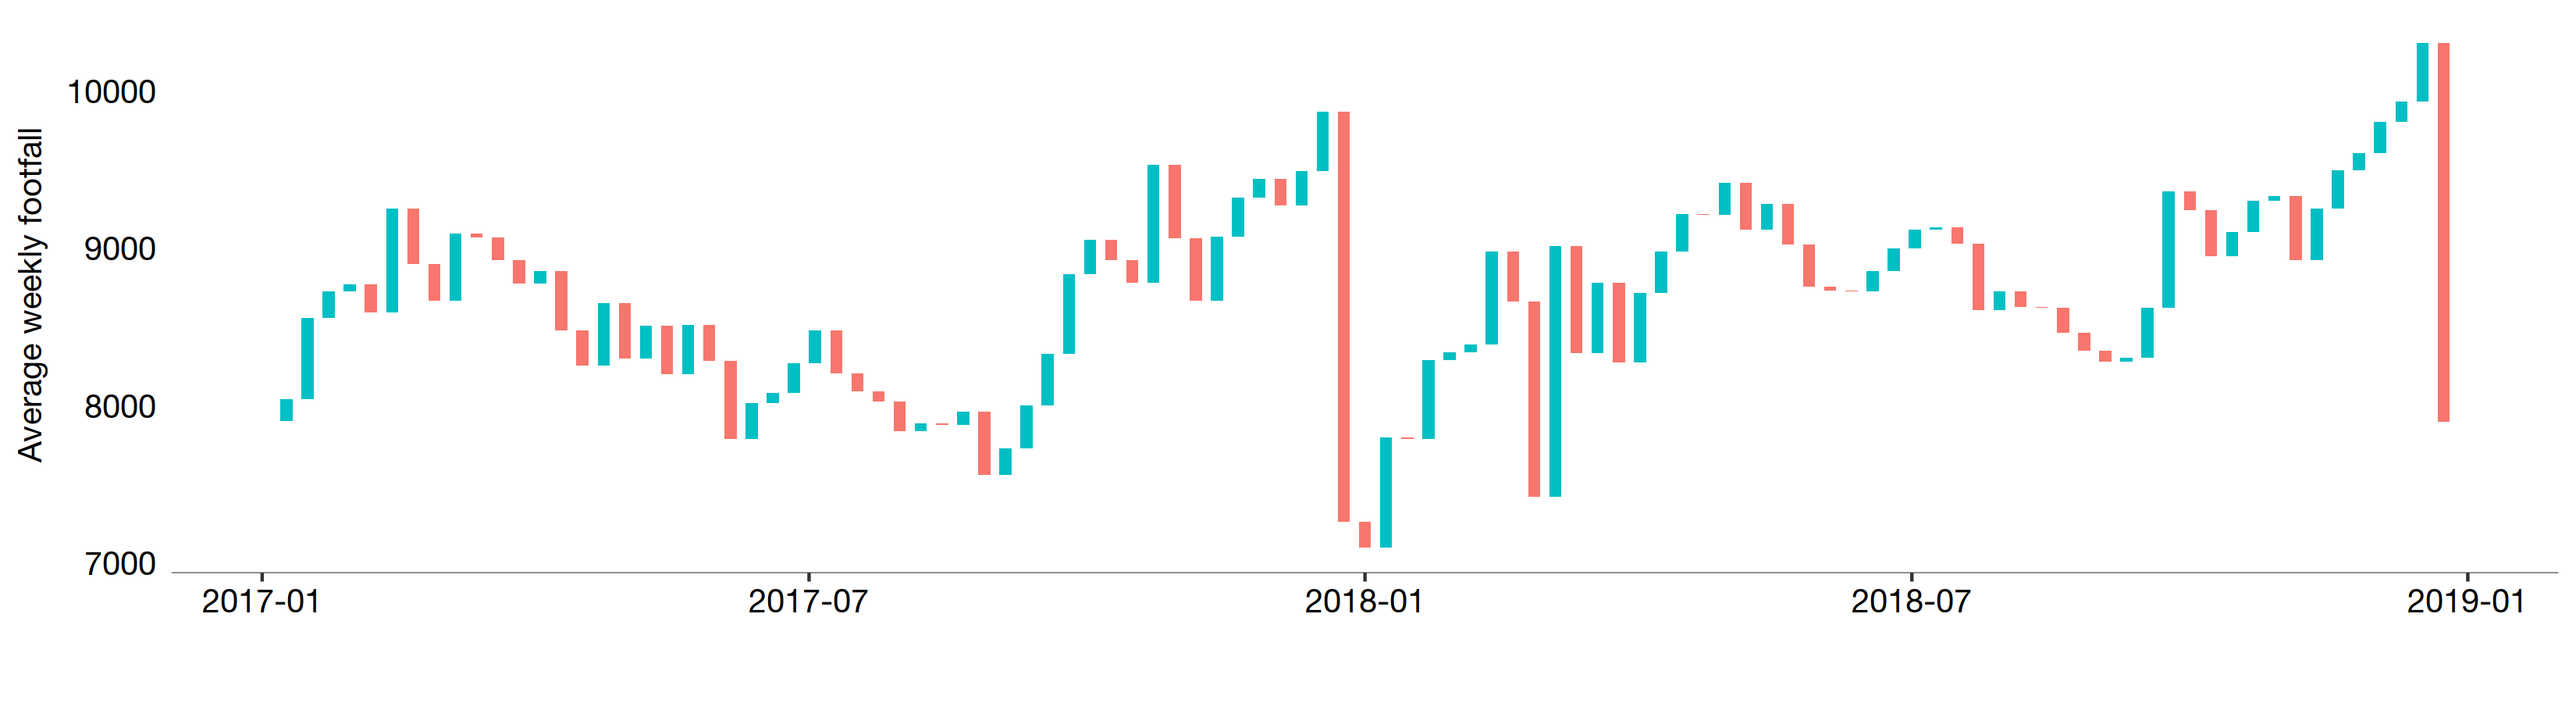
\includegraphics[trim={0 25 0 10},clip]{images/applications-footfall-index.png}
  \caption{A weekly footfall index for United Kingdom showing the change in footfall from 2017 to 18}
  \label{figure:applications:footfall:index}
\end{figure*}

%------------------------------------------------------------------------------%

\cleartoleftpage
\begin{figure*}
  \forceversofloat
  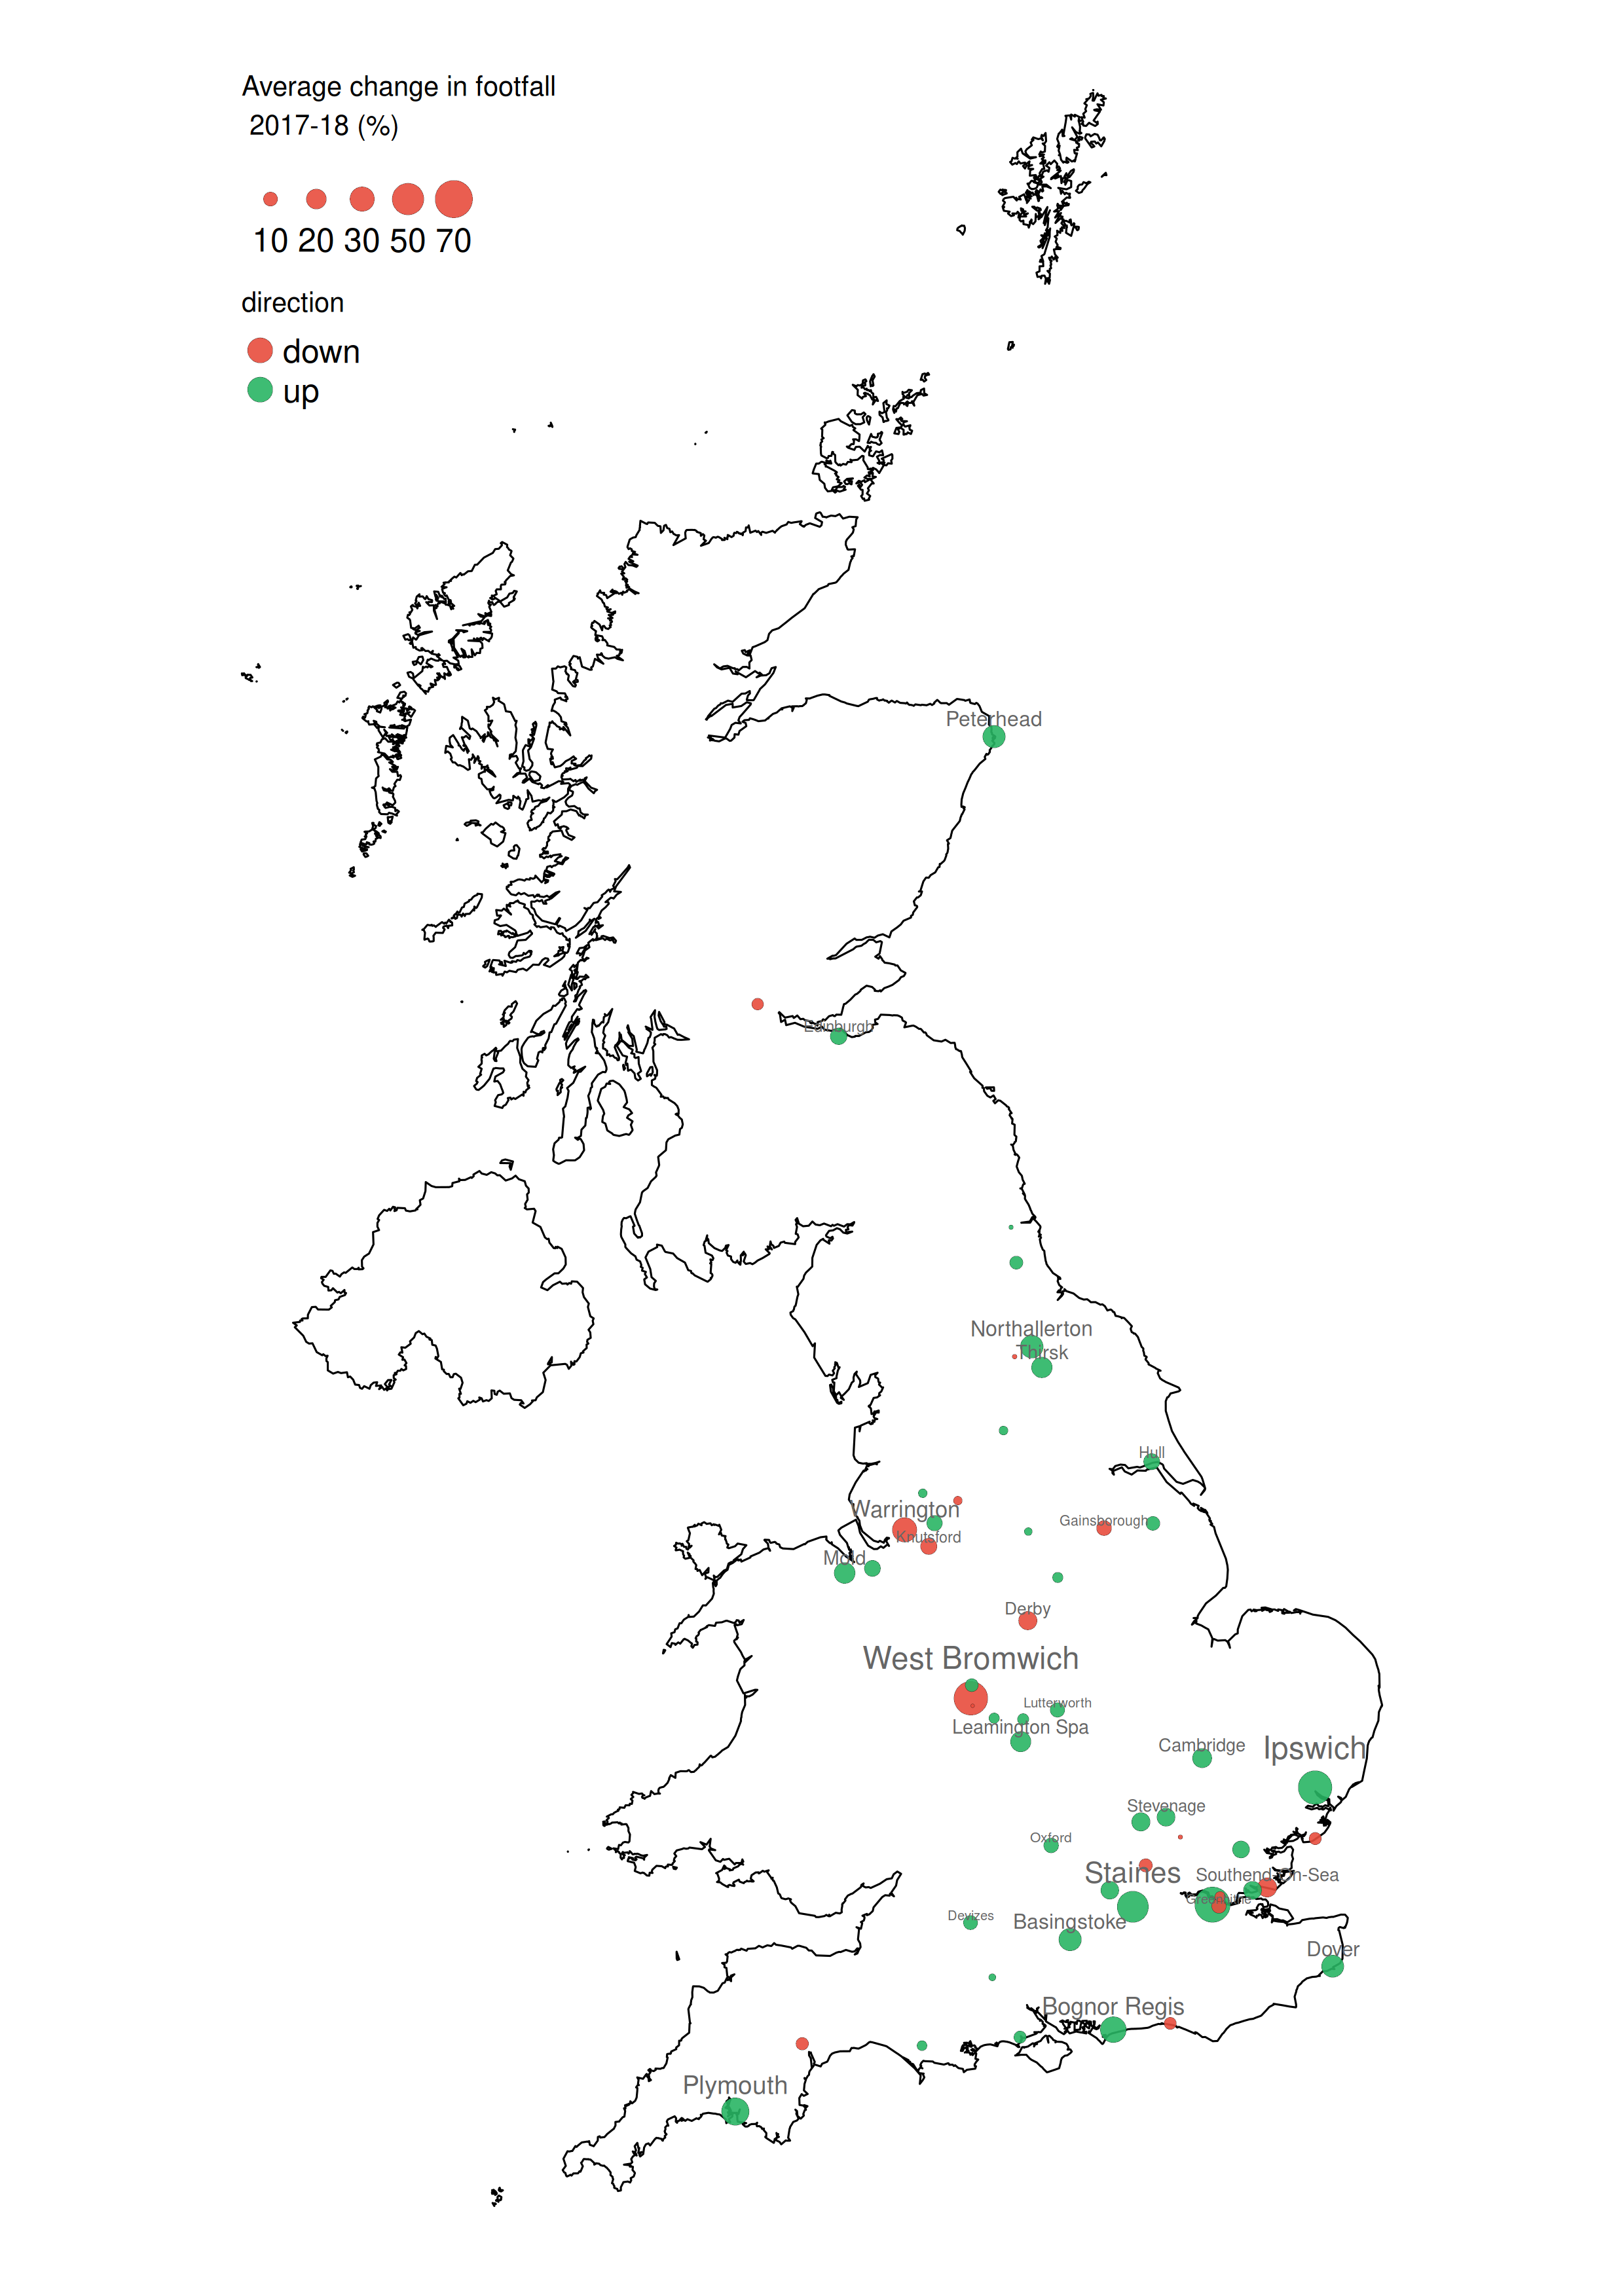
\includegraphics[trim={0 0 0 0},clip]{images/applications-cities-rank.png}
  \caption{The change (\%) in average weekly footfall of towns across UK in 2018 compared to 2017.}
  \label{figure:applications:cities:change}
\end{figure*}

\begin{figure*}
  \forcerectofloat
  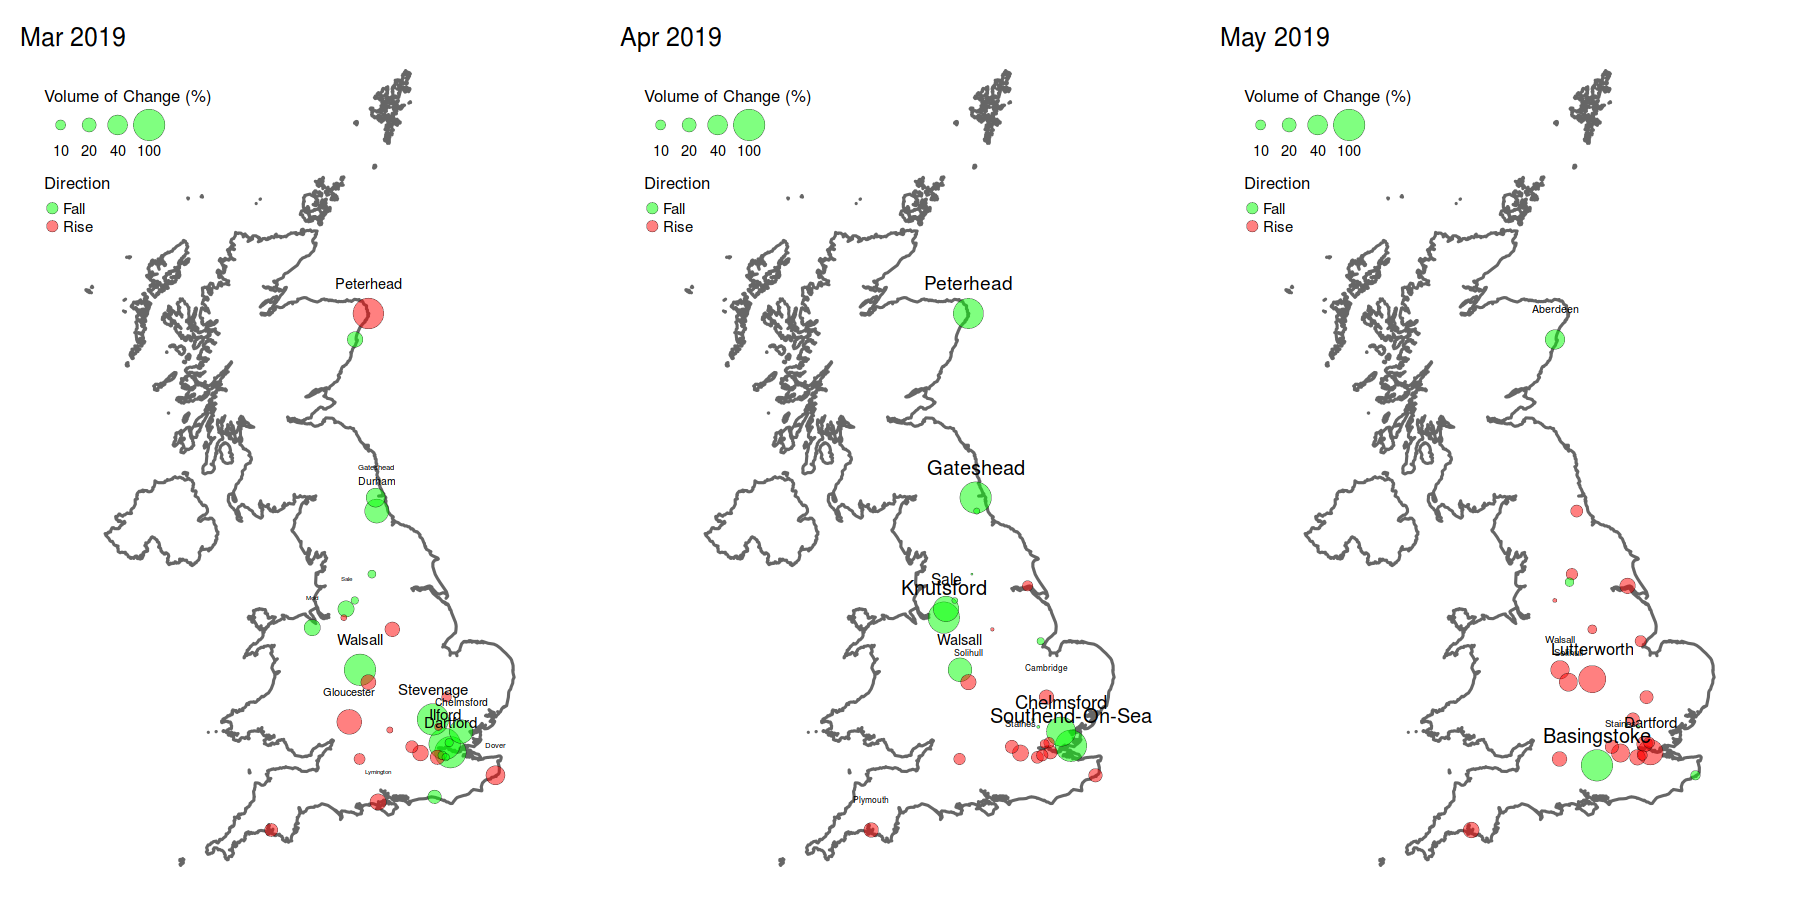
\includegraphics[trim={0 12 0 0},clip]{images/applications-city-indices.png}
  \caption{The change (\%) in monthly average footfall in towns across UK in April and May 2009.}
  \label{figure:applications:cities:month}
\end{figure*}

\begin{figure*}
  \forcerectofloat
  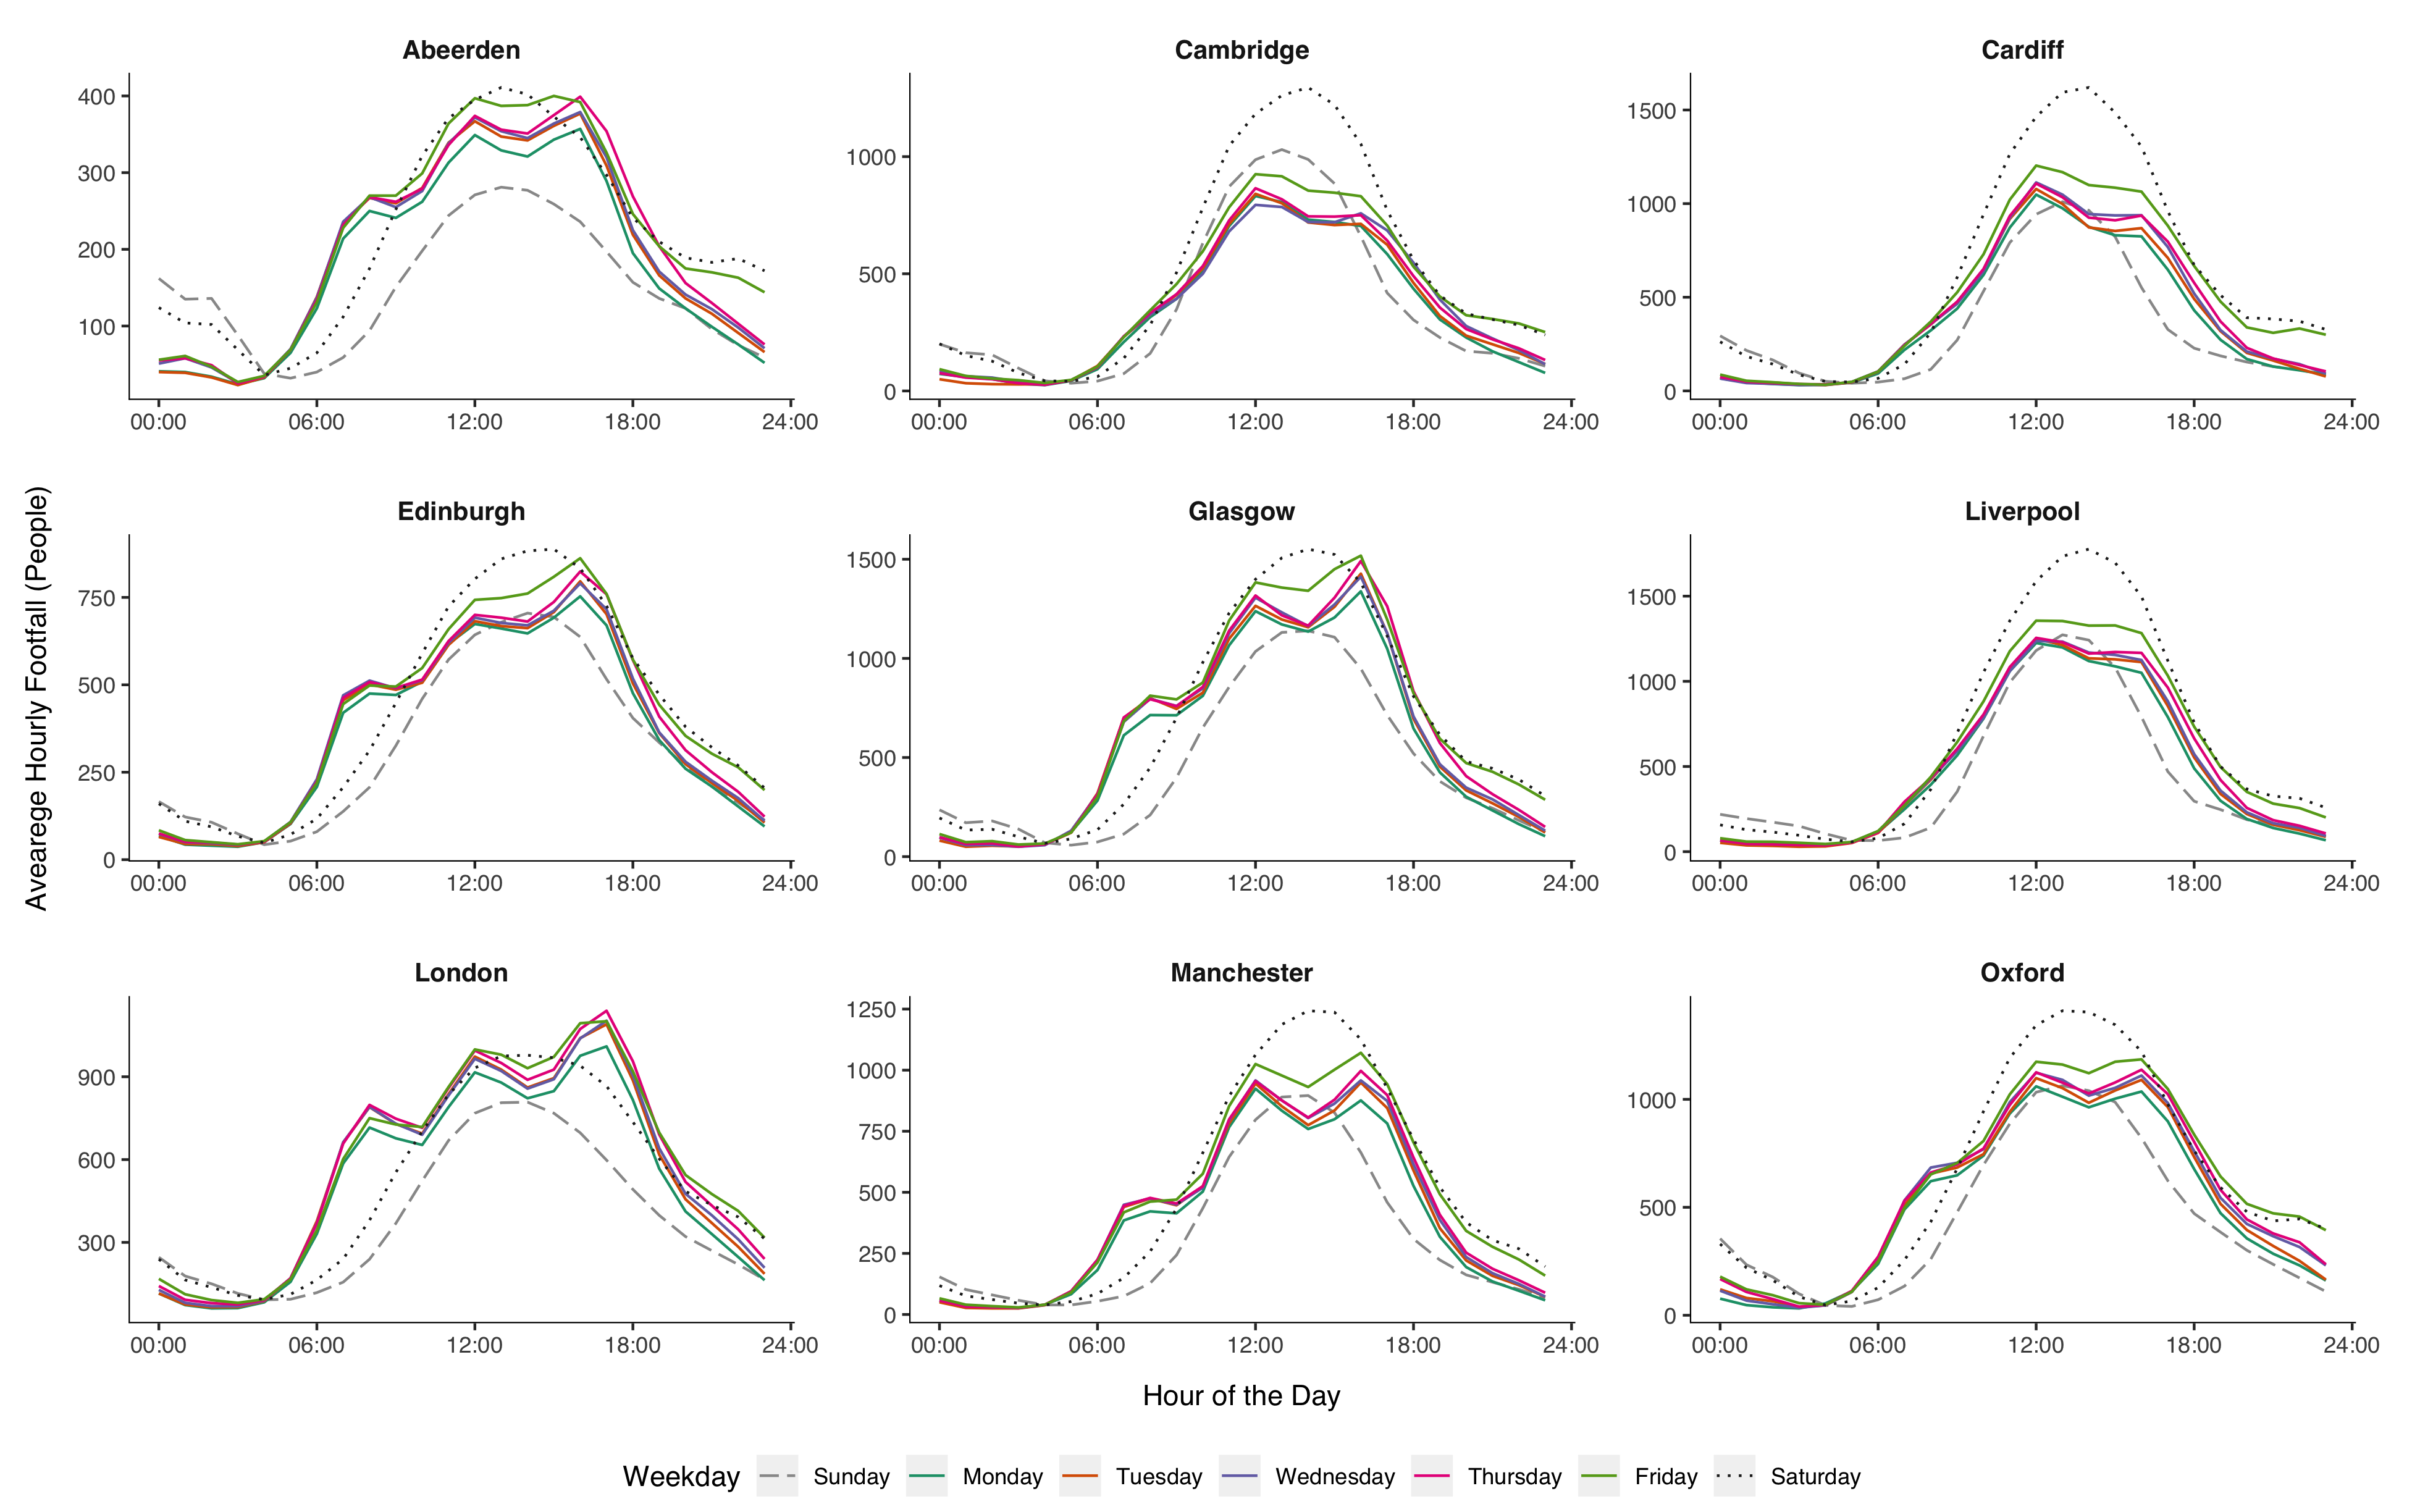
\includegraphics[trim={0 10 0 0},clip]{images/applications-city-profiles.png}
  \caption{Intra-day footfall profile of major cities in United Kingdom}
  \label{figure:applications:cities:profiles}
\end{figure*}

%------------------------------------------------------------------------------%
\cleartoleftpage
\newgeometry{
  left=20mm,
  textwidth=122mm,
  marginparsep=7mm,
  marginparwidth=43mm
}
\begin{figure*}
  \forceversofloat
  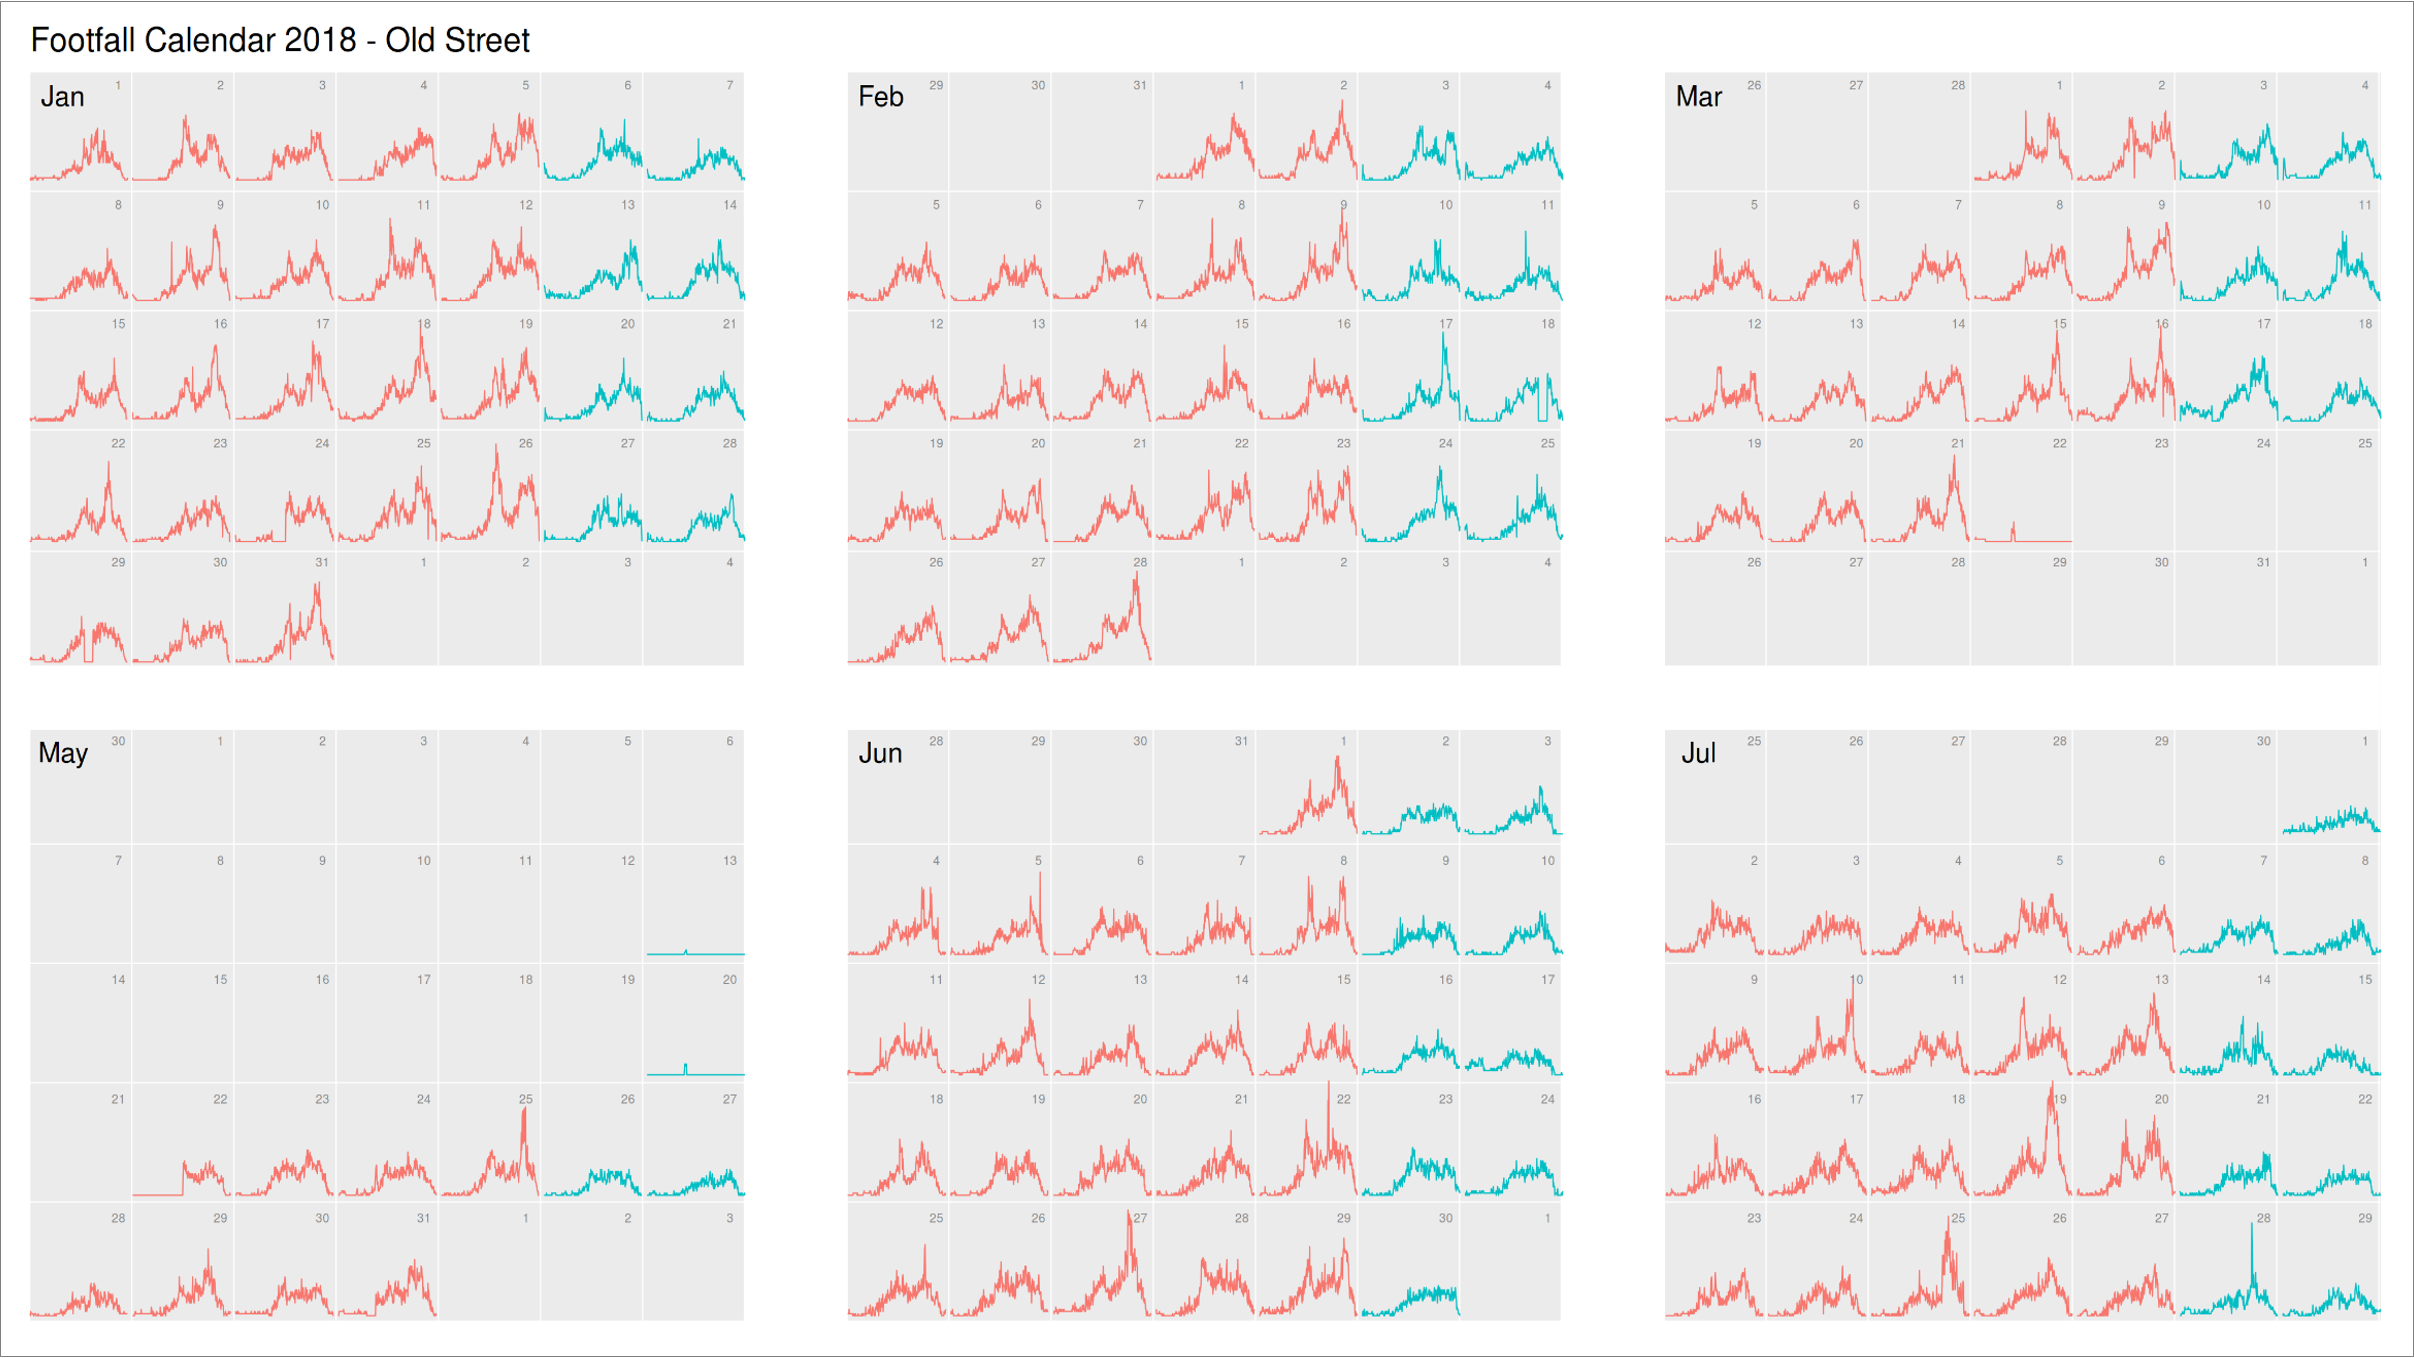
\includegraphics[width=172mm,trim={0 0 1310 -42},clip]{images/applications-footfall-calendar.png}
  \caption{Footfall calendar showing the profiles of daily volume of footfall at Old Street, London.}
  \label{}
\end{figure*}
\clearpage
\begin{figure*}
  \forcerectofloat
  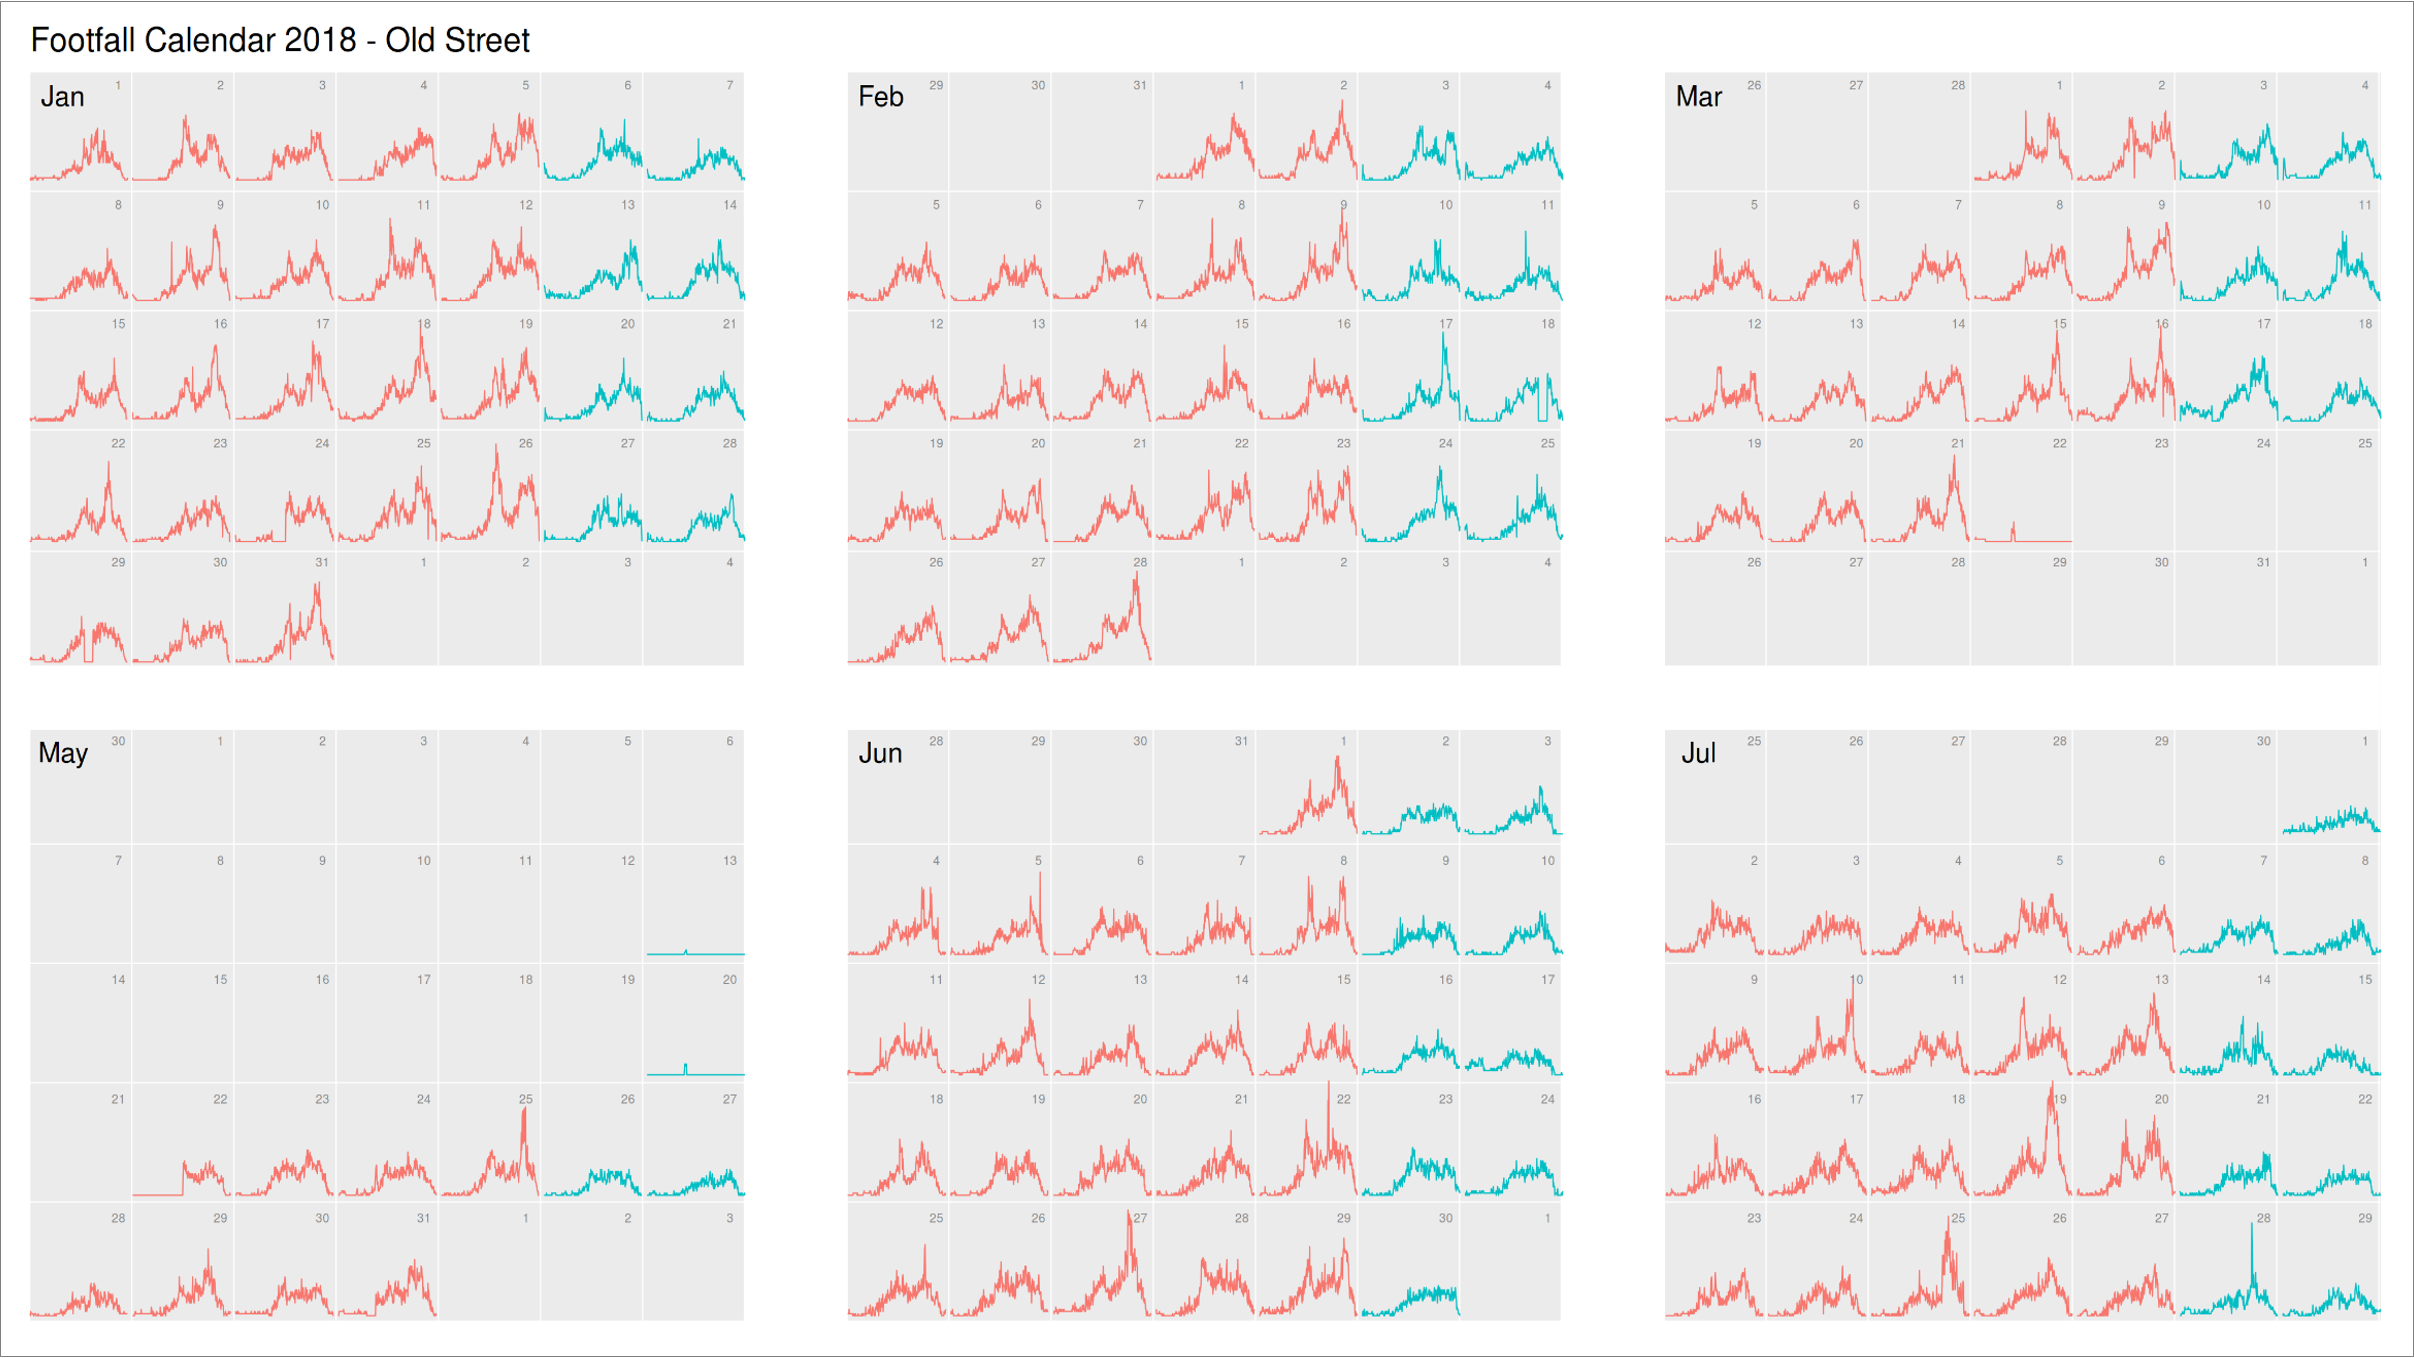
\includegraphics[width=172mm,trim={1315 0 0 0},clip]{images/applications-footfall-calendar.png}
  \caption[]{}
  \label{}
\end{figure*}
\restoregeometry
\clearpage
%------------------------------------------------------------------------------%

\begin{figure*}
  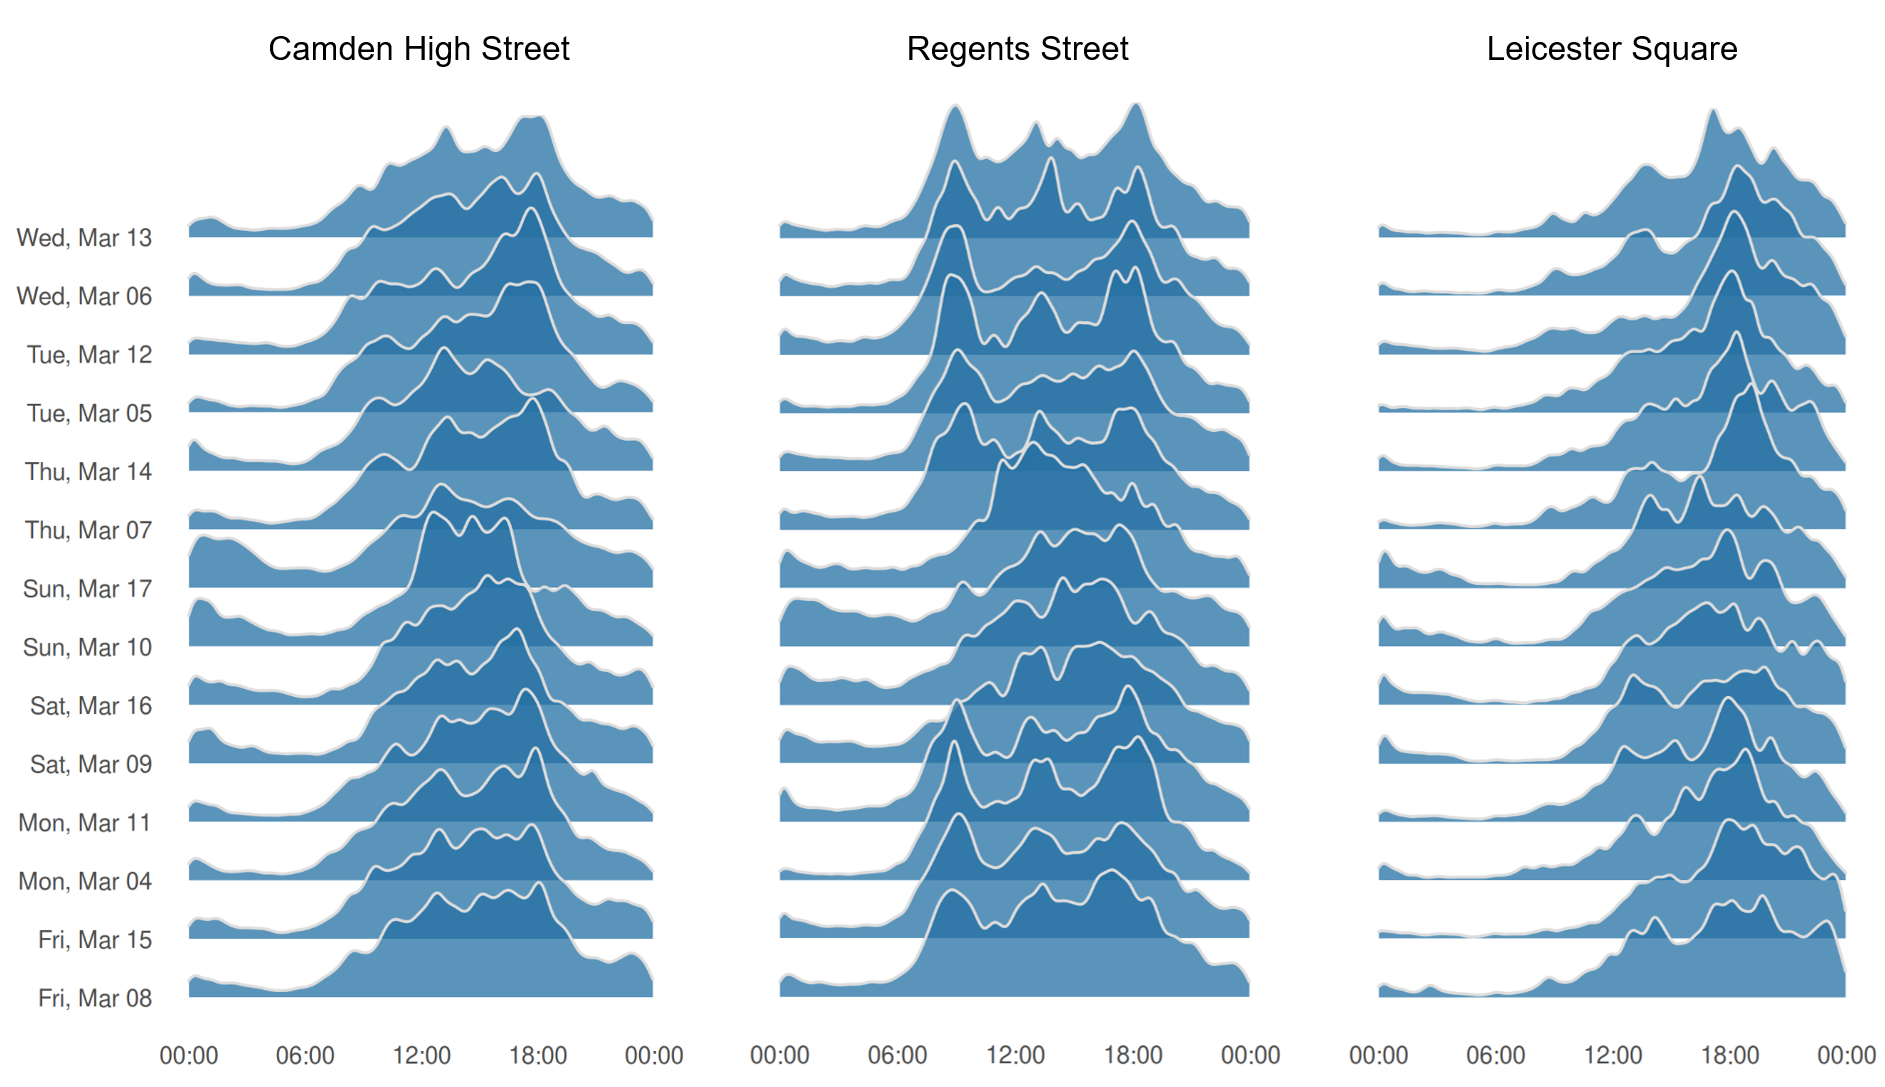
\includegraphics[trim={0 10 0 0},clip]{images/applications-location-profiles.png}
  \caption{The profiles can be tracked longitudinally to reveal nature and change}
  \label{}
\end{figure*}

%------------------------------------------------------------------------------%
\section{Event Detection}
%------------------------------------------------------------------------------%

When footfall is looked at longitudinally across locations, a wide range of information can be uncovered about the context which resulted in the patterns in the footfall. Figure \ref{figure:applications:cardiff} shows the normalised weekly footfall of 10 different locations across Cardiff for two years: 2017 and 2018. The patterns in the footfall clearly show numerous events that were happening in Cardiff as unusually high or low footfall in the corresponding week. The most significant event was in February 2018, when all sensors reported the lowest numbers they have ever recorded. This coincided with the cold wave in UK named ‘Beast from the East’, which brought adverse weather conditions all over the UK and led to a significant reduction in footfall. The other identifiable events are bank holiday weekends which result in higher than normal footfall, and the holiday shopping season when footfall is at its highest. Finally, it is interesting to see the difference in summertime footfall between 2017 and 2018, which could be explained by the FIFA World Cup which took place in the summer of 2018. This example shows the usefulness of the footfall data to detect real life events from the data in near real time. It can also be used to measure the effect of events on footfall, and hence understand the impact of these events for retail and the  economy more generally.

\subsection{Football world cup}
In addition to long-term changes and events, the footfall data can be used to identify the smaller effects of these events at an area scale.
Figure \ref{figure:applications:football} shows footfall from two days in Leicester square, London when the quarterfinal and semifinal matches of the 2018 FIFA World Cup took place. Both matches happened in the evening and led to an  increase in footfall around match time. The most interesting observation is the effect the outcome of the game had on footfall. On the day of the quarterfinal, the winning result of the English team led to a post-match celebration which pushed the Leicester Square footfall to its day-time highest, unlike the day of the semifinal when the English team lost. This not only shows the usefulness of the data in understanding the effect events have on local footfall, but it also shows how the data can be used by retailers to predict the effect the results of sports events might have on them.

\begin{figure*}
  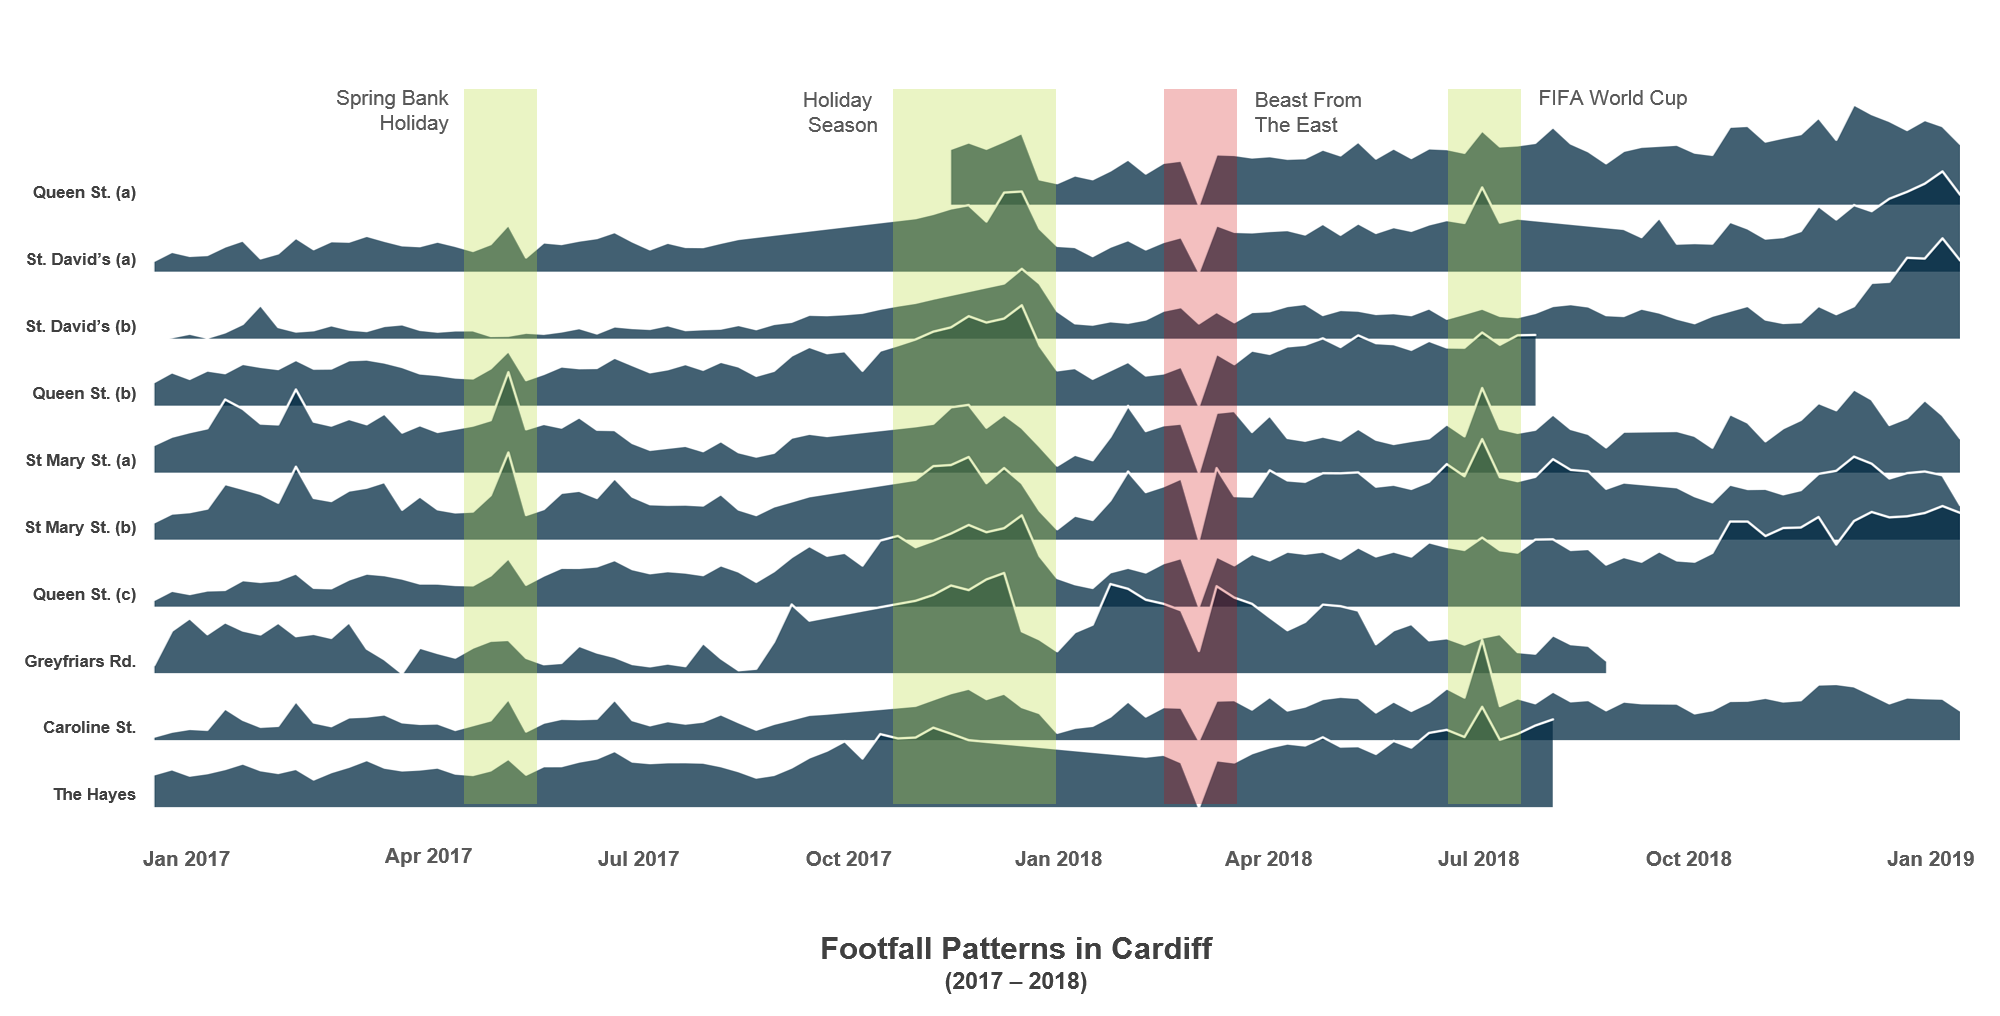
\includegraphics[trim={0 50 0 0},clip]{images/applications-cardiff-footfall.png}
  \caption{Normalised weekly footfall index at locations across Cardiff from 2017 to 2018}
  \label{figure:applications:cardiff}
\end{figure*}

These examples show the importance of footfall data in detecting events. Even a simple visual analytics of the dataset reveal interesting information on events. This would be much more useful when used in tandem with advanced machine learning/data mining techniques, and will predict much better results as more data is collected.

\begin{figure}
  \forceversofloat
  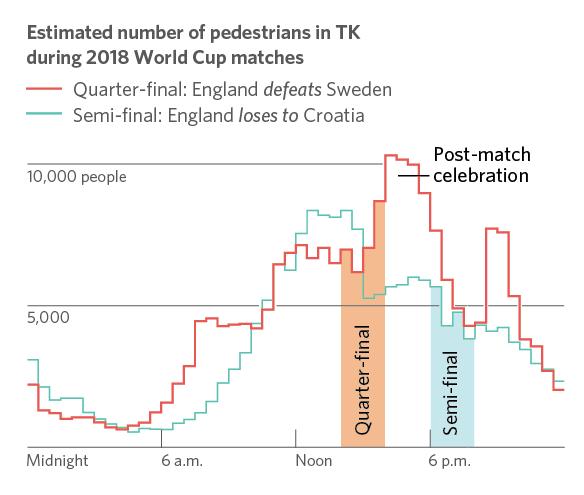
\includegraphics[trim={0 0 0 0},clip]{images/applications-football-sample.png}
  \caption{The difference in footfall distribution at Leicester square, London after FIFA world cup quarter-final and semi-final matches. Source: Oliver Uberti and James Cheshire (Sample needs to be replaced with original graphic)}
  \label{figure:applications:football}
\end{figure}

%------------------------------------------------------------------------------%
\section{Pedestrian Flows}
%------------------------------------------------------------------------------%

Detecting general trends in the flow of people between spatial locations is neither obvious nor a trivial task. This is due the high cost of capturing these movements without compromising people’s privacy, since the primary way to collect such detailed data involves handling people’s precise location data. This research specifically removes any personally identifiable information because of MAC randomisation and hashing, and therefore seems like it might not be suitable for studies on human mobility. However, this problem can be solved by examining the movement of people in the Smart Street Sensors network at a fine spatial and temporal resolution using a novel methodology in the field of Big Data which uses mathematical models from information theory: Transfer Entropy (TE). Using an area in central London, this section serves as a case study to demonstrate the usefulness of TE as a measure of the flow of pedestrians.

\sidenote{Work done is collaboration with Roberto Murcio and Karlo Lugomer. The methodology was formulated by Roberto, the author worked on the implementation of the method on the case study.}

Consider the array of sensors shown in Figure \ref{figure:applications:transent} and assume that there is a flow of people walking past Location 116 and then diffusing towards the remaining sensors. Counts generated by the sensor are aggregated per five minute intervals, so if, for example, it takes one minute to walk from Location 116 to Location 117, the number of people detected at 117 from minutes 2 to 5, would correspond to the percentage of people detected at 116 from minutes 1 to 4. In other words, the similarity between the time series of counts at the locations under consideration are correlated. Hence the aim here is to provide a measure for the size of the flow between each pair of sensors without actually tracking individual people. One way to accomplish this, is to think of this motion of people as flows of information among distinctive sources, so we can relate the number of people reaching one sensor from another by measuring the uncertainty between two interacting random variables. For this, we used an information theory concept known as Transfer
Entropy (TE) defined by:

\begin{equation} \label{equation:te}
  TE(X,Y) = \sum_{t=1} p(y_{t+1}, y_{t}, x_{t}) \times { log{ \frac{p(y_{t+1} \mid y_{t}, x_{t})}{p(y_{t+1} \mid y_{t})}} }
\end{equation}

Where $t$ indicates a given point in time.
Equation \ref{equation:te} measures the reduction in uncertainty at $y_{t}$, given $x_{t}$ and $y_{t-1}$.
In comparison with the case when only $y_{t-1}$ is known.
This measure is applied directly to our people's movement problem and $X$ = location i, $Y$ = location j and $t$ runs for a whole day, the $TE$ would represent an indicator for the direction of the flow, as the counts at $y_{t+1}$ are more accurately estimated using the information of $x_{t}$.

\begin{figure*}
  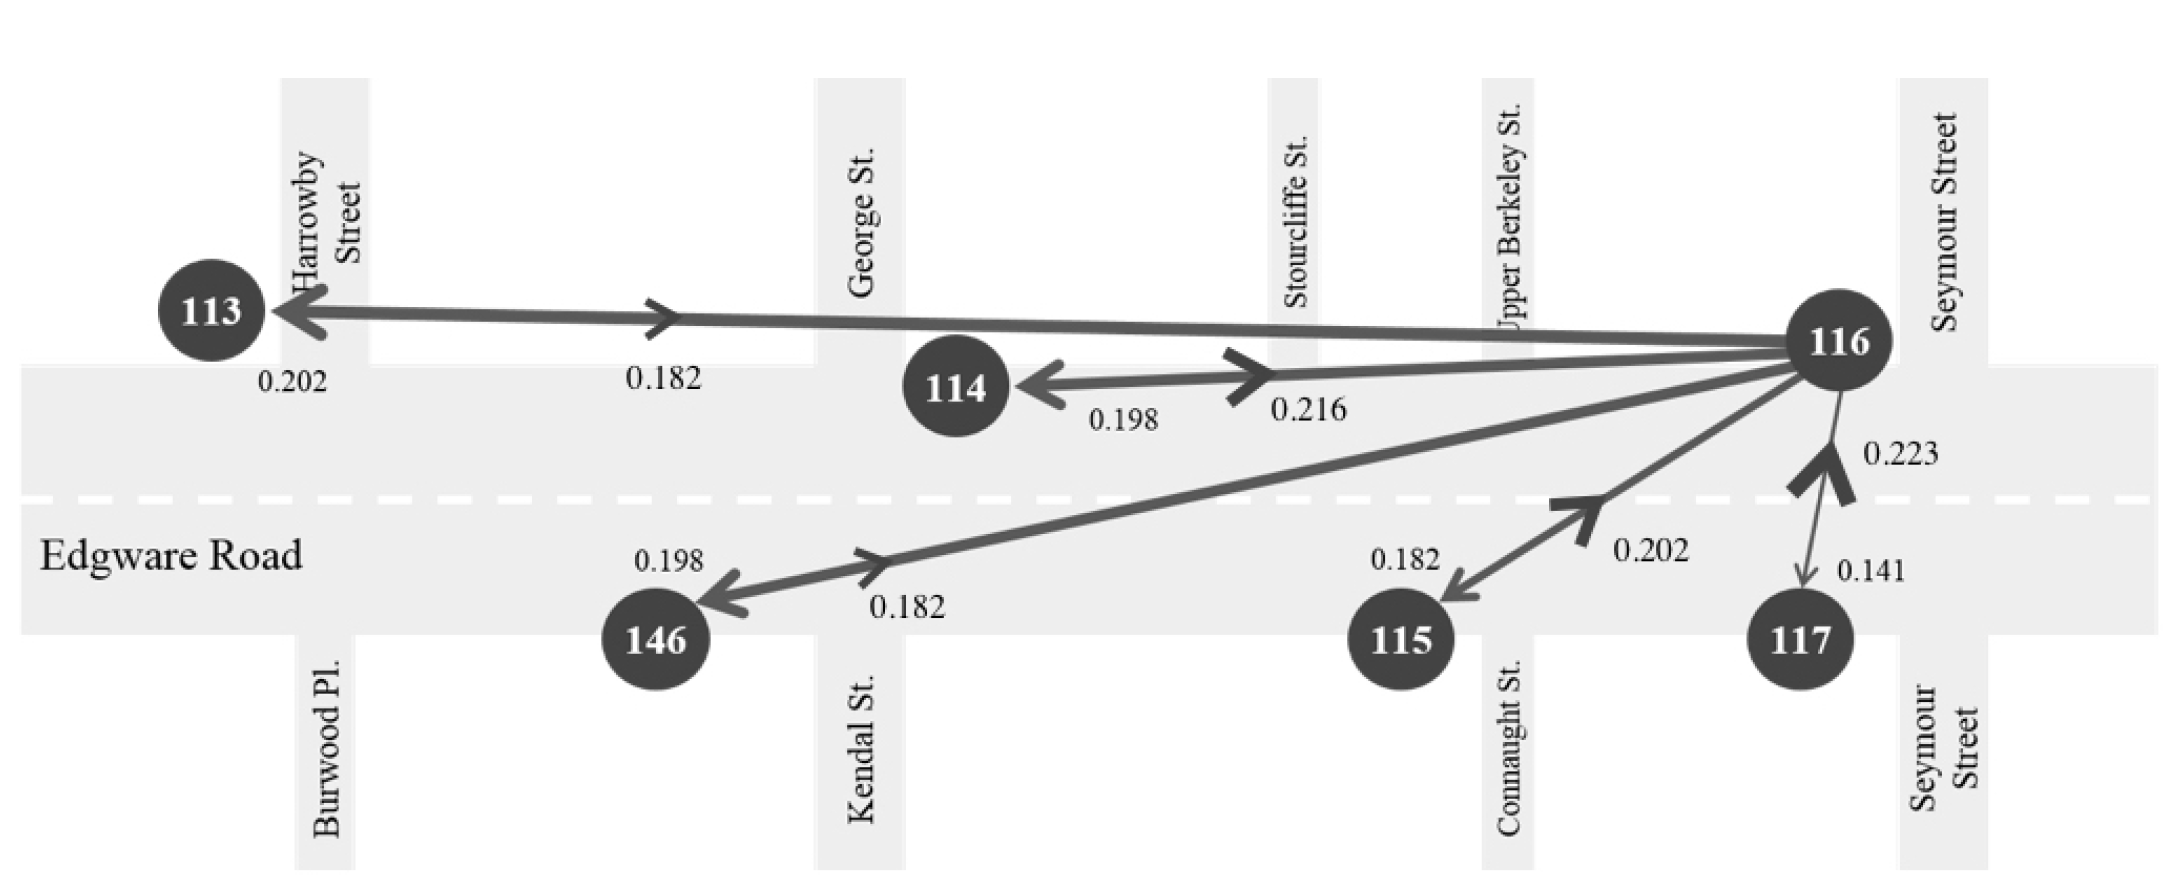
\includegraphics[trim={0 0 0 0},clip]{images/applications-transfer-entropy.png}
  \caption{Illustration of transfer entropies between set of locations along Edgware Road, London.}
  \label{figure:applications:transent}
\end{figure*}

Taking again Figure \ref{figure:applications:transent} as a reference, we measured the $TE$ between sensor 116 and the rest of the sensors.
The walking time is not constant and each sensor has counts at all times $i$, $j$.
There are people passing by these sensors that came from locations outside the network.
The numbers at each line represent the $TE$ measured between each pair of sensor locations.
The largest $TE$ value found was between 117 and 115.
The asymmetry of the TE is clear here, as the value in the opposite direction (115 to 117) is considerably lower.
Another interesting value is the pair 116-117, where TE(116,117) << TE(117,116).
This demonstrates that in this four-way crossing, the predominant direction of flow is from Location 117 to Location 116 (from the bottom of the figure upwards, or from west to east in reality). These results suggest that, in general, there is a larger flow of people from the west side to the east side of Edgware Road, and a larger flow of people from south to north of it. The results are consistent with our intuition that there is a larger flow of people from south to north along this road towards Edgware Road underground station.

There is still a series of uncertainties yet to be addressed by this model, such as the decay of probabilities with distance and the number of interventions of opportunity encountered by people while walking from one sensor to another.
However, this first initial set of results is encouraging in measuring flow between spatial points without actually tracking these users.
